\chapter{66 kV Network Representation in RSCAD and PowerFactory}

\section{Single OWF 66 kV network, Draft module in RSCAD}

\begin{figure}[H]
\centering
%\hspace*{-0.2cm}
    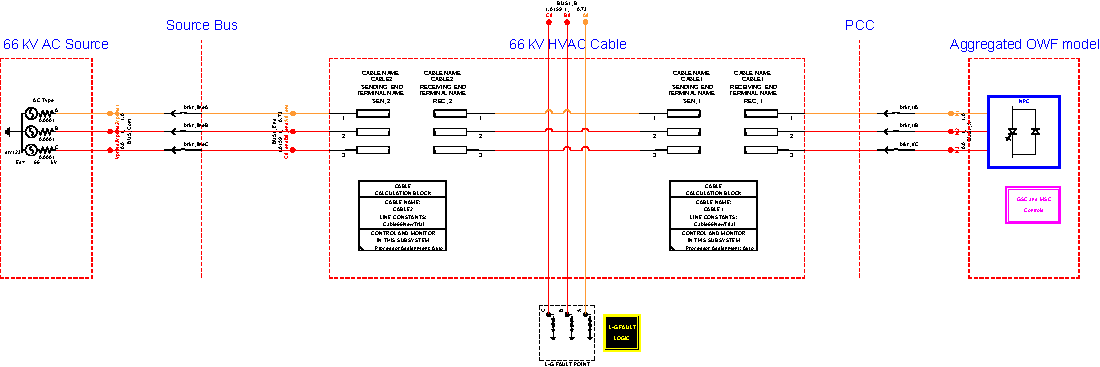
\includegraphics[height = 6cm,width = \textwidth]{Diagrams/Appendix_B/WT1_AC_RSCAD_network_view.pdf}
    \caption{66 kV HVAC test system representation in Draft module in RSCAD}
    \label{fig:WT1_AC_RSCAD_network_view}
\end{figure}

\section{Single OWF 66 kV network, Runtime module in RSCAD}
\begin{figure}[H]
\centering
%\hspace*{-0.2cm}
    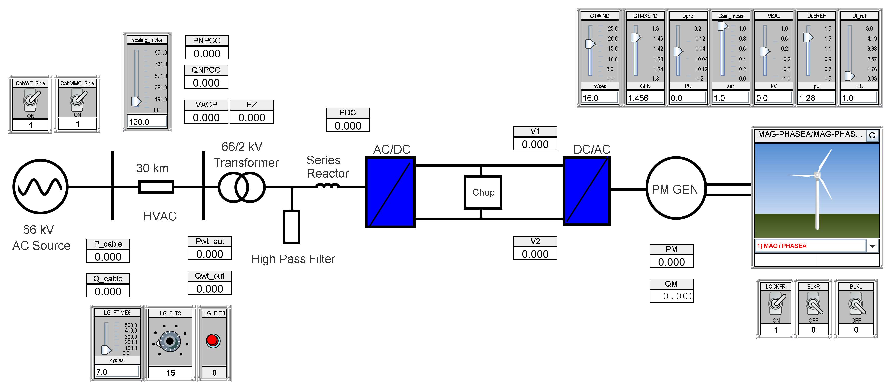
\includegraphics[height = 7cm,width = 16.5cm]{Diagrams/Appendix_B/WT1_AC_RSCAD_network_sib_view.pdf}
    \caption{66 kV HVAC test system representation in Runtime module in RSCAD}
    \label{fig:WT1_AC_RSCAD_network_sib_view}
\end{figure}

\section{Single OWF 66 kV network in PowerFactory}
\begin{figure}[H]
\centering
%\hspace*{-0.2cm}
    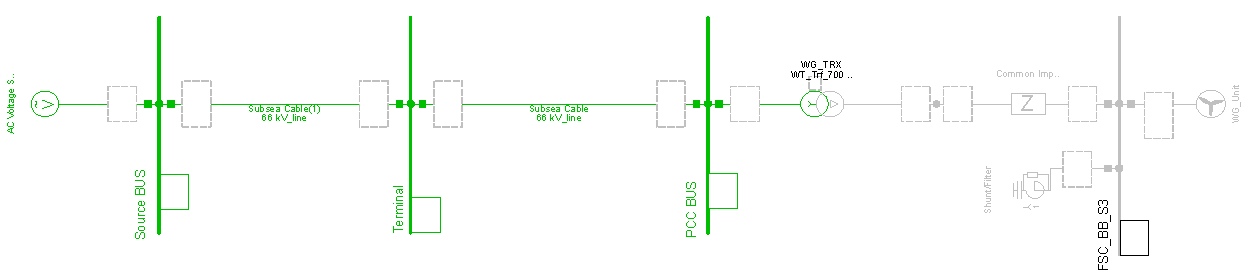
\includegraphics[height = 5cm,width = 17.5cm]{Diagrams/Appendix_B/WT1_AC_PFD_network_view.pdf}
    \caption{66 kV HVAC test system representation in PowerFactory}
    \label{fig:WT1_AC_PFD_network_view}
\end{figure}

\section{Additional graphs}
\subsection{Three-phase line to ground fault in the middle of the cable}

\begin{figure}[H]
%\centering
%\hspace*{-1.2cm}
    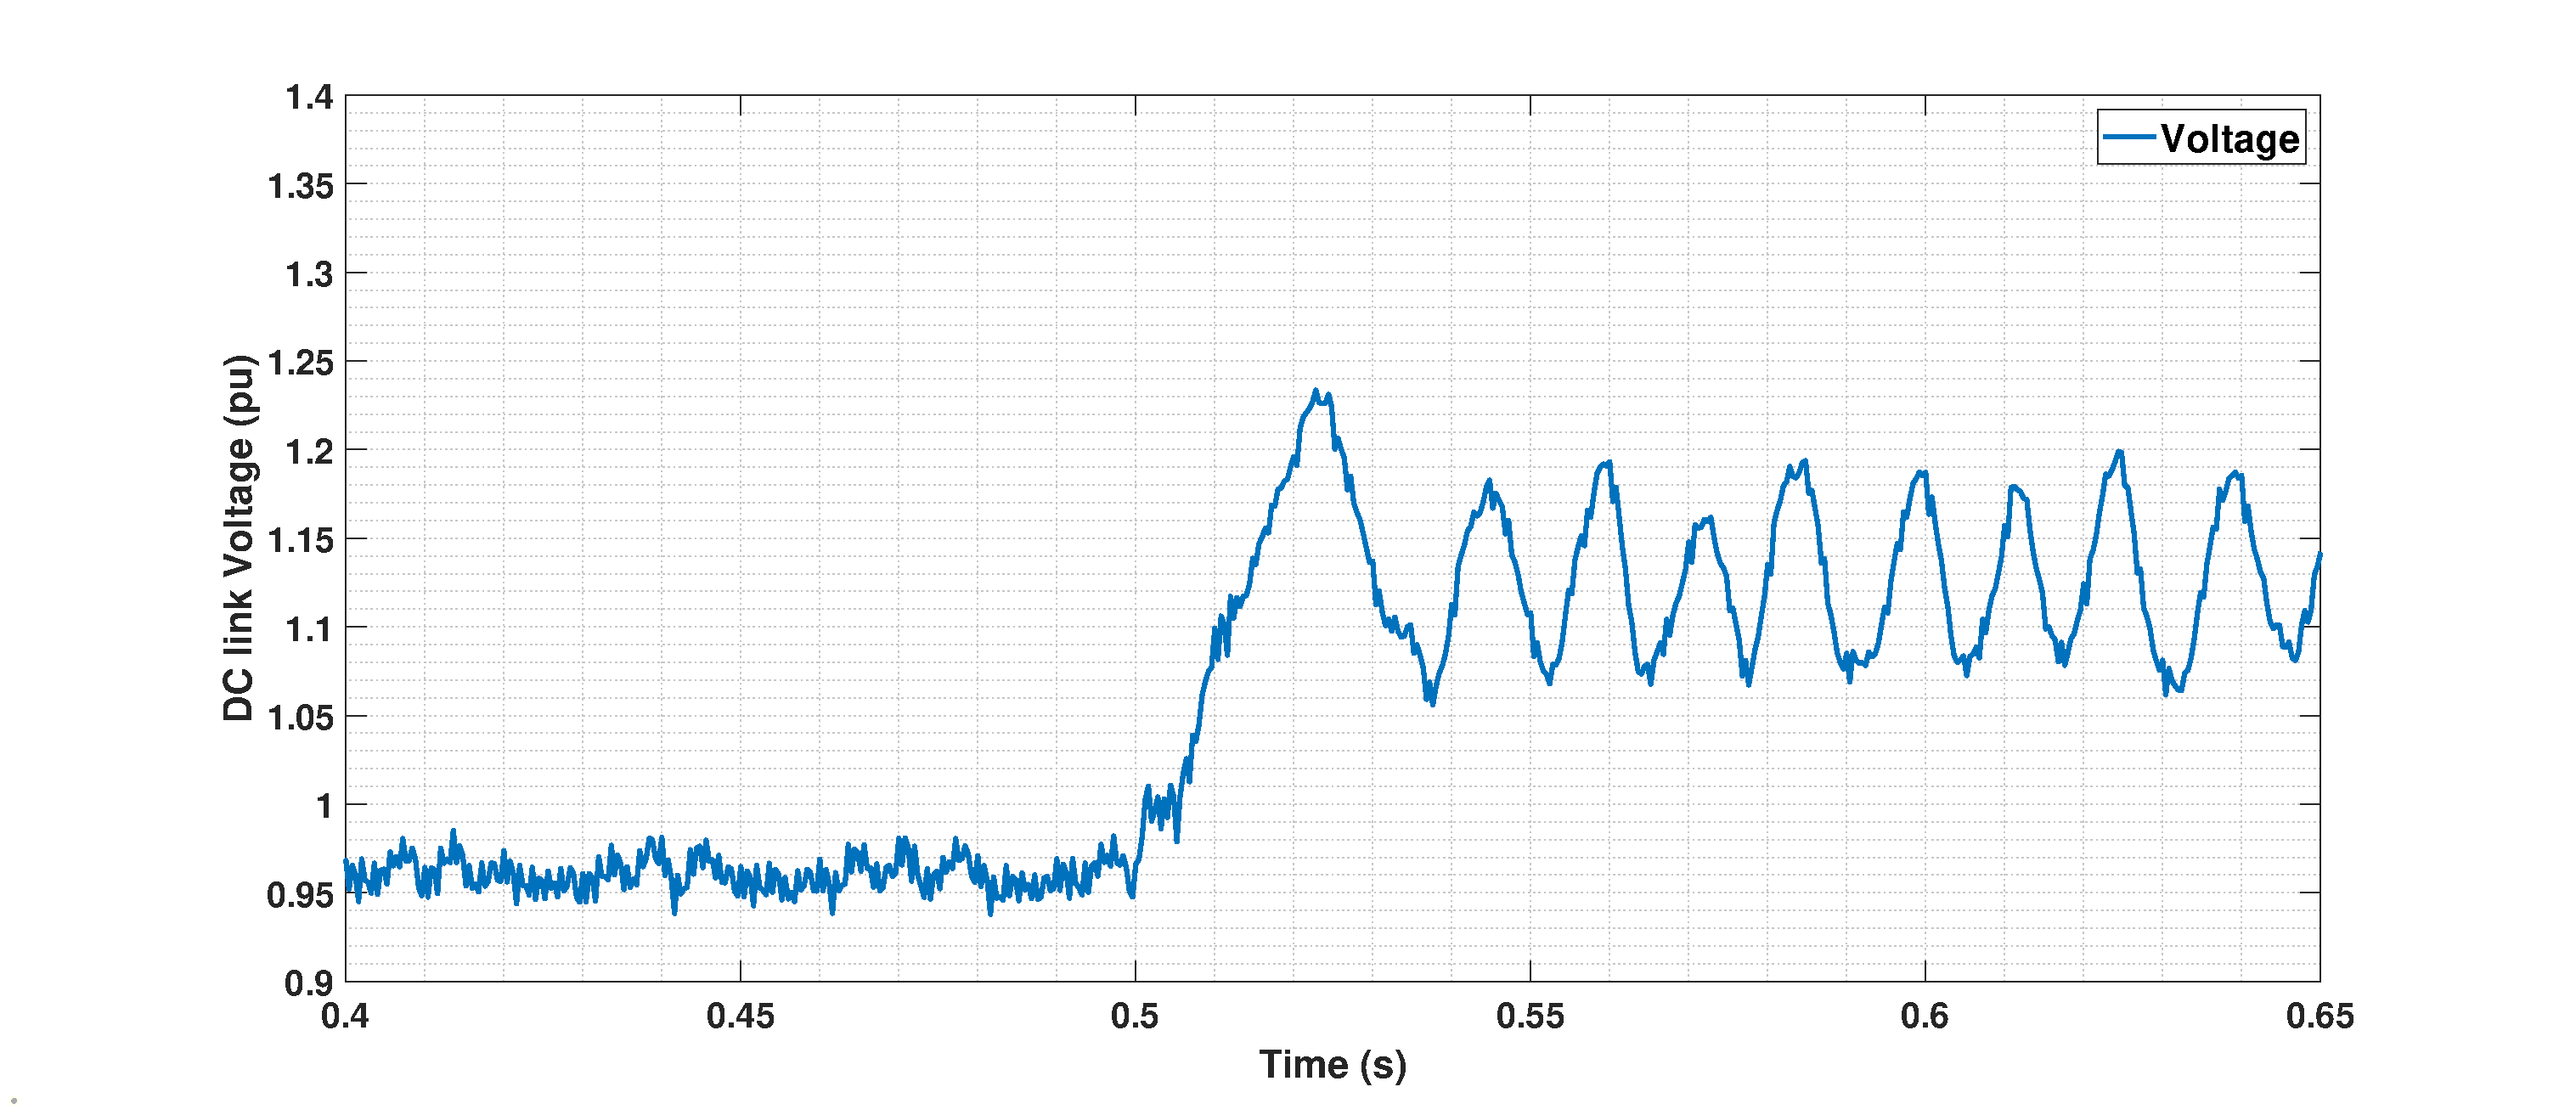
\includegraphics[height = 7cm,width = \textwidth]{Diagrams/Appendix_B/DC_Voltage_RSCAD.eps}
    \caption{Voltages at DC link upon three-phase line to ground fault in the middle of cable in RSCAD}
    \label{DC_Voltage_RSCAD}
\end{figure}

\begin{figure}[H]
%\centering
%\hspace*{-1.2cm}
    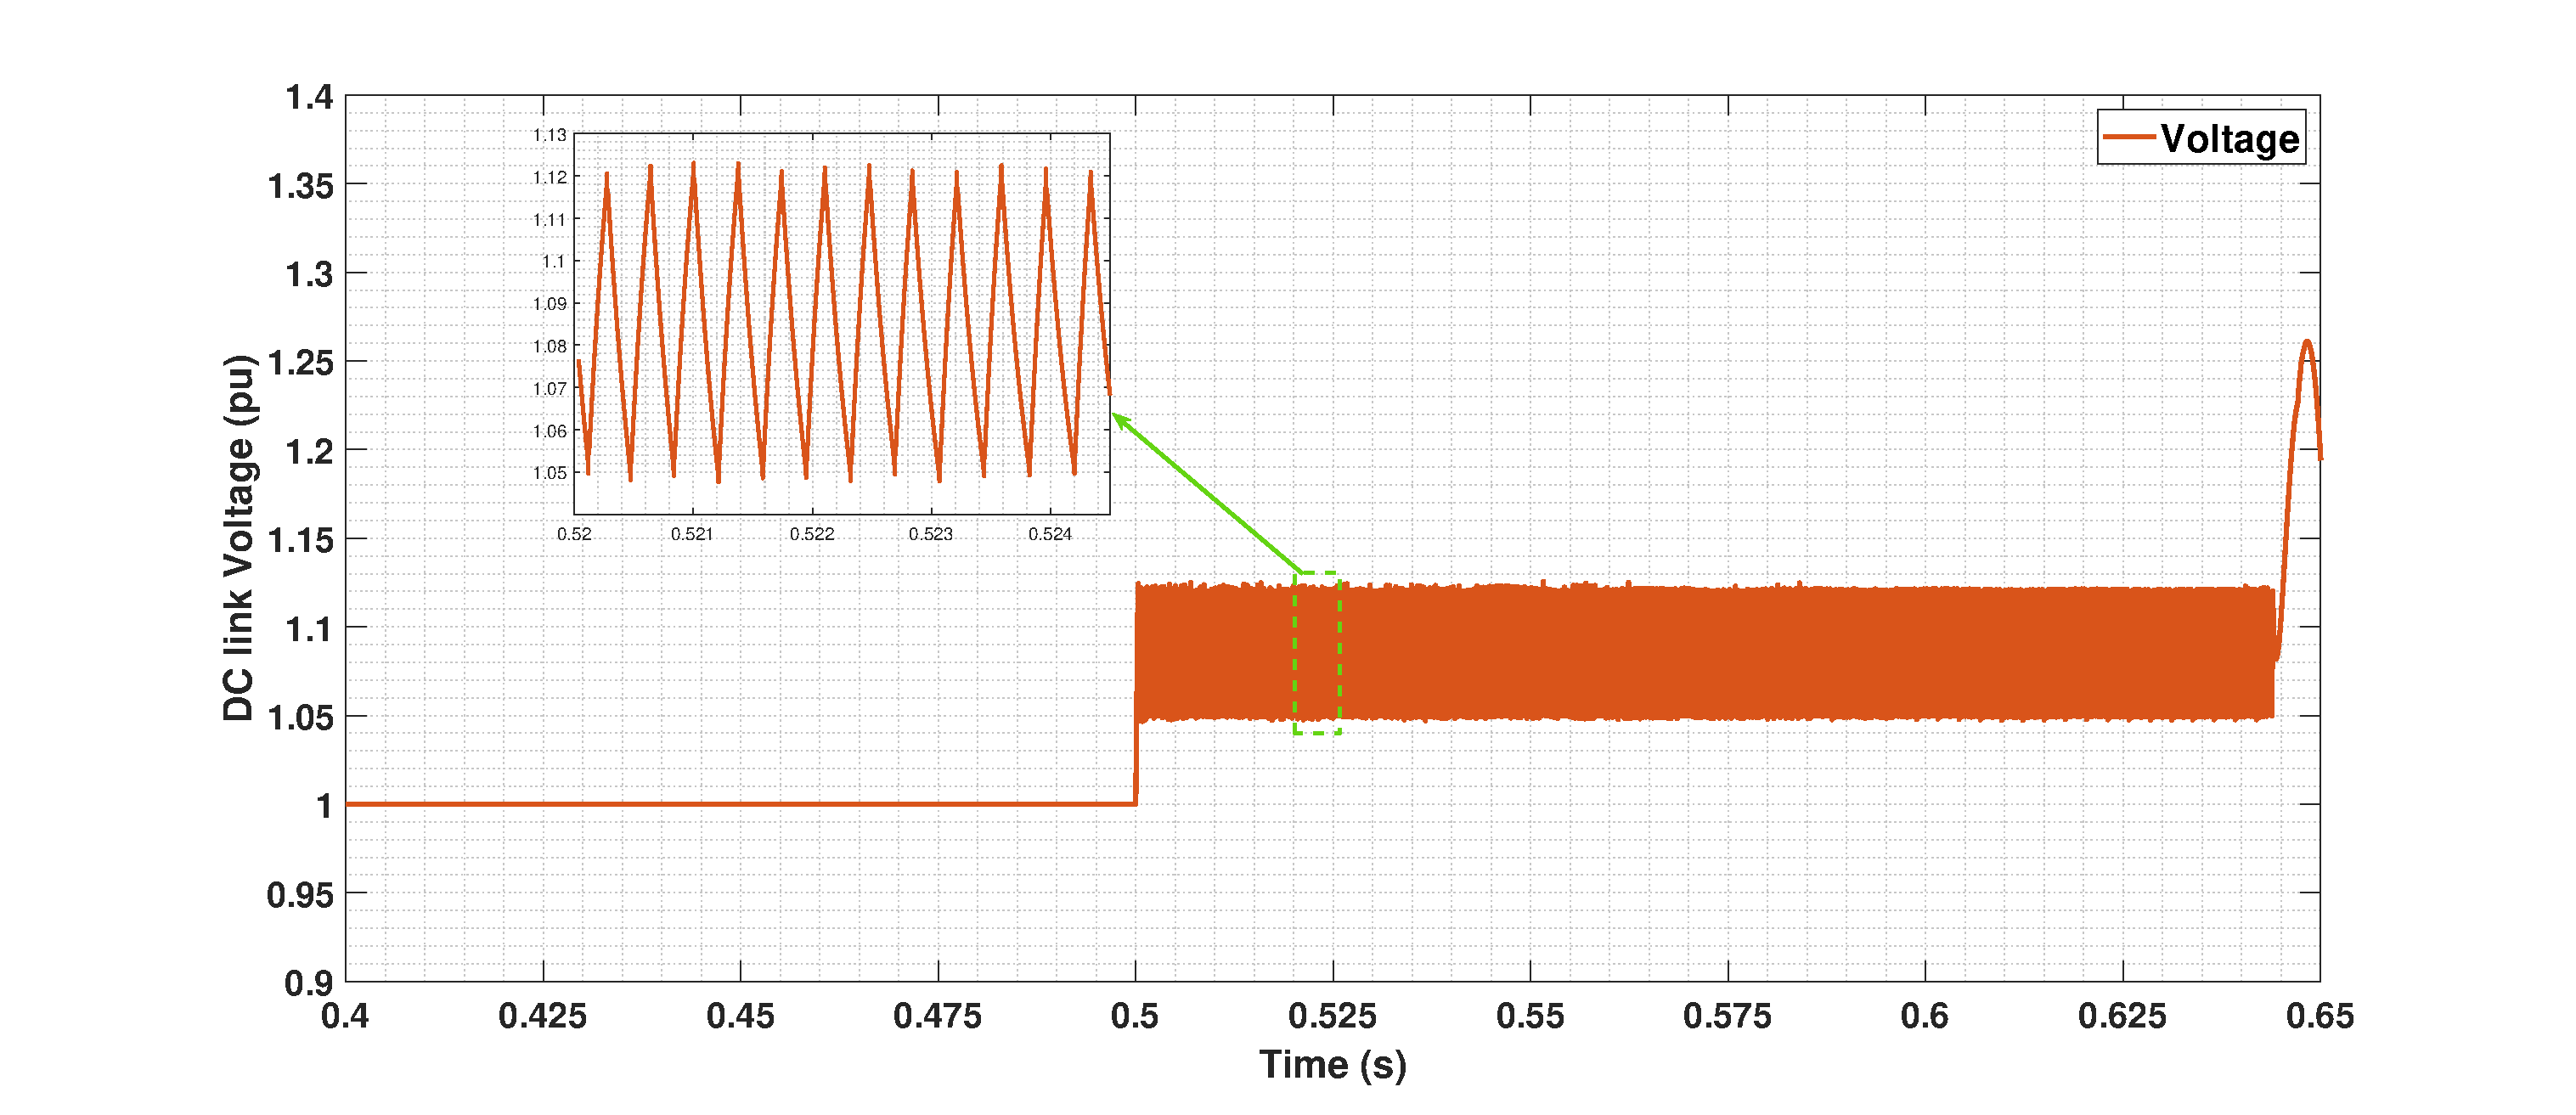
\includegraphics[height = 7cm,width = \textwidth]{Diagrams/Appendix_B/DC_Voltage_PFD.eps}
    \caption{Voltages at DC link upon three-phase line to ground fault in the middle of cable in PowerFctory}
    \label{DC_Voltage_PFD}
\end{figure}

During the time of fault, the \gls{DC} link voltage increases as seen in the Figures \ref{DC_Voltage_RSCAD} and \ref{DC_Voltage_PFD}. The chopper gets activated when the voltage goes above 1.05 p.u. in both the models. However, switching of the chopper depends on the time delay of the signal given to the triangular wave repeater in the RSCAD model. Whereas, the hysteresis block shown in Figure \ref{fig:DC_bus_PFD} determines the activation of the chopper in the PowerFactory model. 
